\documentclass[usenatbib]{mn2e}

\usepackage{graphicx}
\usepackage{subfigure}

\begin{document}

\title{Modelling circumstellar discs with 3D radiation hydrodynamics}
\author[David M. Acreman, David A. Rundle, Tim J. Harries]{David M. Acreman, David
  A. Rundle, Tim J. Harries\\
School of Physics, University of Exeter, Stocker Road, Exeter EX4
4QL. E-mail acreman@astro.ex.ac.uk
}

\maketitle

\begin{abstract}

We present results from combining a grid-based radiative transfer code
with a Smoothed Particle Hydrodynamics code to produce a flexible
system for modelling radiation hydrodynamics. The system is tested
using a benchmark model of a circumstellar disc. We find that the SED
and temperature distribution within the disc are highly sensitive to
the representation of the disc inner edge, which depends critically on
both the grid and SPH resolution. The system is then used to model a
circumstellar disc around a T-Tauri star and is found to produce a
steady state disc in both hydrostatic and radiative equilibrium. 

\end{abstract}

\begin{keywords}
hydrodynamics -- radiative transfer -- methods: numerical
\end{keywords}

\section{Introduction}

The interaction between matter and radiation is of great importance in
a range of astrophysical processes. A major challenge in star
formation simulations is to incorporate self-consistent radiative
feedback from protostars. Once this is achieved it is possible to
relax the simplifying assumptions relating to the equation of state
and to study the effects of radiative feedback, for example the impact
on disc fragmentation. A flux limited diffusion approximation can be
used to represent radiative transport in regions of high optical
depth, however this method is not suited to modelling regions of low
optical depth where an alternative method, such as a Monte-Carlo
method, must be used.

This paper presents a results from coupling the {\small{TORUS}} radiative
transfer code \citep{harries_2000} with the SPH (Smoothed Particle
Hydrodynamics) code of \cite{bate_2009}.  {\small{TORUS}} performs radiative
transfer calculations using the Monte-Carlo method of \cite{lucy_1999}
with a flux limited diffusion approximation in regions of high optical
depth. The radiative transfer calculations are performed on a grid
which uses adaptive mesh refinement (AMR) to allow variable
resolution.  The SPH method is well suited to dealing with the large
range in size scales encountered during star formation processes, hence
an SPH code coupled to a combined Monte-Carlo and flux limited
diffusion radiative transfer code is a very flexible method for
performing star formation calculations incorporating radiative
feedback.

There is not a unique approach to coupling an SPH code to a radiative
transfer code and a number of different approaches have been developed
(\cite{nayakshin_2009}, \cite{pawlik_2008} and references
therein). This paper focuses on radiative transfer calculations using
an adaptive grid in the context of modelling processes in star
formation.

Accurately coupling the SPH component to the radiative transfer
component requires an effective transformation from the Lagrangian
particle description of SPH to the Eulerian grid description of an AMR
grid. The procedure used for this transformation is tested using a
benchmark case (see Sections~\ref{section:description_of_benchmark}
and~\ref{section:grid_generation}). The spectral energy distribution
and temperature distribution of the benchmark disc are examined in
Section~\ref{section:seds} in order to understand how well the
radiative transfer calculation works with the gridded density field
and to understand the effects of grid and SPH spatial resolution. A
simulation of a circumstellar disc around a T Tauri star is presented
in Section~\ref{section:sph_disc} with the aim of calculating an
equilibrium state in three dimensional hydrostatic and radiative
balance.

\section{Circumstellar disc benchmark}
\label{section:description_of_benchmark}

When constructing validation tests of a numerical method it is often
valuable to use a simplified test case with well known results. We
base our SPH disc benchmark on the axisymmetric circumstellar disc of
\cite{pascucci_2004}.  Representing a structure with rotational
symmetry using a 3D geometry allows us to validate the operation of
our method against well tested results from other codes while fully
exercising the 3D capabilities of our own system.

The density of the disc benchmark described by \cite{pascucci_2004} is
given by
\begin{equation}
\rho\left(r,z\right) = \rho_0 \left( \frac{r}{r_d} \right)^{-1} \exp
\left( - \frac{\pi}{4} \left( \frac{z}{h\left(r \right)}  \right)^2 \right)
\label{eqn:pascucci_density}
\end{equation}
where $r$ is the distance from the central star in the mid-plane and
$z$ is the height from the mid-plane. The expression $h\left( r
\right)$ is given by
\begin{equation}
h\left( r \right) = z_d \left( \frac{r}{r_d}\right)^{1.125}  
\end{equation}
and $\rho_0$, $z_d$ and $r_d$ are constant parameters.  We base our
benchmark model on the most optically thick case presented by
\cite{pascucci_2004} which has a mid-plane optical depth of $\tau=100$
at $\lambda=550~\rm{nm}$ and a mass of 0.011~$\rm{M}_{\sun}$. This
requires $r_d=500~\rm{AU}$, $z_d=0.25 r_d$ and
$\rho_{0}=8.1614\times10^{-18}~\rm{g~cm^{-3}}$, with the disc truncated at
an outer radius of 1000~AU and an inner radius of 1~AU.

The benchmark disc is implemented using an ensemble of equal mass SPH
particles. If all the particles have the same mass then the number
density is proportional to the mass density, hence the SPH particles
sample a probability density distribution such that the probability of
finding a particle in a given volume is proportional to the mass in
that volume as a fraction of the total mass \citep{gingold_1977}. 
Hence the analytical density function can be converted into a
probability function which describes the probability of finding a
particle in a given volume.  An ensemble of particle positions can
then be calculated by randomly sampling the probability density
functions for $r$ and $z$ and assigning a uniformly random spherical
polar angle $\theta$. The particle's density is set to the value given
by Eqn~\ref{eqn:pascucci_density} based on the particle's position.

Each particle is assigned a smoothing length $h_{\rm{smooth}}$ given by 
\begin{equation}
h_{\rm{smooth}} = 1.2 \left( \frac{m_{\rm{part}}}{\rho_{\rm{part}}} \right) ^{1/3}
\end{equation}
where $m_{\rm{part}}$ is the particle mass and $\rho_{\rm{part}}$ is
the particle density, according to the method of
\cite{price_2008}. The smoothing length is used when reconstructing
properties represented by the ensemble of particles, for example the
density distribution on the radiative transfer grid is 
constructed using a kernel smoothing method (see
Section~\ref{section:grid_generation}).

\section{Generation of adaptive grid from SPH-particles}

\label{section:grid_generation}

An important step in setting up grid-based radiative transfer using
SPH particles is determining an effective transformation of the
required model fields (e.g. density) between the SPH particle
representation and the grid representation.  The representation on
grid should preserve important properties of the SPH model, e.g. total
mass and density gradients. This section determines a grid
construction method which allows a good degree of control over the
number of cells in the grid while maintaining an accurate
representation of the density distribution.

\subsection{Grid generation method}

{\small{TORUS}} uses an adaptive grid based on the octree method. In a 3D
geometry the initial grid comprises 8 cells (one octal) with 2 cells
in each dimension. An algorithm is applied to determine whether to
split each cell into a further 8 cells, similar to the method of
\cite{kurosawa_2001}. The properties of the adaptive grid are
determined by a combination of the algorithm used to decide when to
split a cell and the method used to assign density values to cells.

The density in a given grid cell is calculated using a kernel
smoothing method. The kernel smoothed density is normalised by the sum
of the kernel weights, if the sum of the weights is greater than 0.3,
to ensure a smooth density distribution within the interior of the
disc. If the sum of the weights is less than 0.3 then the density is
not normalised by the sum of the weights, in order to avoid numerical
effects at the free surface as described by \cite{price_2007}.  The
method used to construct an AMR grid from SPH particles is described
in more detail in \cite{rundle_2009}.

\subsection{Grid generation tests}

Two grid splitting conditions were tested. The first method splits a
grid cell if the mass within the cell exceeds a given limit. For this
condition the resolution is highest where the density is highest
(i.e. resolution increases towards the disc mid-plane and towards the
centre of the disc) which is analogous to the effective spatial
resolution of SPH.  The second condition decides whether to split the
cell based on the fractional density difference between the most dense
and least dense SPH particles contained within the cell. The quantity
\begin{equation}
f_{\rm{split}}=\frac{\rho_{\rm{max}} - \rho_{\rm{min}}}{\rho_{\rm{max}} + \rho_{\rm{min}}}
\end{equation}
is calculated, where $\rho_{\rm{max}}$ is the highest SPH particle
density and $\rho_{\rm{min}}$ is the lowest SPH particle density, and
the cell is split if a specified value of $f_{\rm{split}}$ is
exceeded. 

To illustrate the effects of the different splitting methods two
example grids are shown in Fig.~\ref{fig:example_meshes}. A grid
constructed from $10^7$ particles, using a mass per cell limit of
$5\times10^{26}~\rm{g}$, is plotted in
Fig.~\ref{fig:mass_condition_mesh}. This plot is a slice along $y=0$
showing the grid in the $x$-$z$ plane and shows the increased
resolution towards the disc centre and mid-plane.  A grid with 
$f_{\rm{split}}=0.1$, also using $10^7$ particles, is plotted in
Fig.~\ref{fig:density_condition_mesh}. The resolution is highest at
the edge of the disc, where there are large density gradients, and the
resolution also increases towards the centre of the disc.
\begin{figure*}
  \subfigure[AMR grid with a mass per cell condition of
    $5\times10^{26}~\rm{g}$.]
    {\includegraphics[scale=0.22]{figures/set1_mesh}
  \label{fig:mass_condition_mesh}}
  \subfigure[Grid with a density condition of
    $f_{\rm{split}}=0.1$.]
    {\includegraphics[scale=0.22]{figures/set2_mesh}
      \label{fig:density_condition_mesh}}
  \caption{Example AMR grids for a mass per cell splitting condition (left)
    and a density contrast splitting condition (right). In both cases
    $10^7$ particles were used. The axis units are $10^{16}$~cm.}
  \label{fig:example_meshes}
\end{figure*}

For each splitting condition a number of AMR grids were generated
using different values of the mass per cell limit or
$f_{\rm{split}}$. This was repeated for discs represented by $10^5$,
$10^6$ and $10^7$ SPH particles. Figure~\ref{fig:grid_tests} plots the
number of octals generated as a function of mass per cell or
$f_{\rm{split}}$ (solid line), and the percentage error in the disc
mass (dashed line). The percentage error in disc mass is calculated by
comparing the total mass on the AMR grid with the known mass of
$0.011~\rm{M}_{\sun}$ based on the analytical form of the density
distribution, and a positive value indicates that mass on the grid is
too large. In all cases the total mass obtained by summing the masses
of all SPH particles is correct to within a factor of $10^{-8}$.
\begin{figure*}
  \subfigure[Mass per cell condition and $10^5$ particles]{\includegraphics[scale=0.3]{figures/1e5_set1}}
  \subfigure[Mass per cell condition and $10^6$ particles]{\includegraphics[scale=0.3]{figures/1e6_set1}}
  \subfigure[Mass per cell condition and $10^7$ particles]{\includegraphics[scale=0.3]{figures/1e7_set1}}
  \subfigure[Density contrast condition and $10^5$ particles]{\includegraphics[scale=0.3]{figures/1e5_set2}}
  \subfigure[Density contrast condition and $10^6$ particles]{\includegraphics[scale=0.3]{figures/1e6_set2}}
  \subfigure[Density contrast condition and $10^7$ particles]{\includegraphics[scale=0.3]{figures/1e7_set2}}
  \caption{Number of octals (solid line) and percentage mass error
    (dashed line) for AMR grids generated using different grid
    splitting methods and different numbers of particles. }
  \label{fig:grid_tests}
\end{figure*}

The mass per cell condition allows a wide range in the total number of
octals while maintaining a total mass which is correct to within a few
percent. The number of octals as a function of mass per cell limit is
consistent between runs with different numbers of SPH particles, apart
from the case with $10^5$ particles and a mass limit of
$10^{26}$~g. In this case the mass per cell limit is smaller than the
SPH particle mass and the grid is over sampling the SPH resolution. In
the other cases the mass per cell limit is greater than the SPH
particle mass. For mass per cell limits of $10^{28}$g and less the
total mass error varies only slowly as a function of mass per
cell. There is a positive bias in the total mass but using more SPH
particles results in a more accurate total mass. 

If a density contrast condition is used then the total number of
octals depends on the number of particles, unlike in the mass per cell
case. The general form of the number of octals as a function of
density contrast is the same in all three cases but the normalisation
varies substantially. In order to ensure a total mass accurate to with
1~per~cent the density contrast condition would require at least $10^7$
particles and a density contrast threshold of no more than 0.3.

The density contrast condition is effective in adding extra resolution
in regions of high density contrast (see
Fig.~\ref{fig:density_condition_mesh}) but has a less robust total
mass representation than the mass per cell limit. By using a
combination of these two conditions it is possible to add extra
resolution in high contrast regions and still maintain an accurate
total mass.
 
\section{Temperature distribution and SED generation}

\label{section:seds}

Ensuring a consistent representation of mass and density in the grid
representation and in the SPH representation is an important
requirement in ensuring accurate radiative transfer calculations. In
order to have confidence in the results of the calculations we must
also ensure that the temperature distribution is realistic. By
comparing the Spectral Energy Distribution (SED) from our disc with the
benchmark results we have a global measure of how well the density and
temperature distributions are represented. In order to get an accurate
SED both the density and temperature distributions must be well
represented.

The disc was initially modelled using $10^5$ SPH particles and a mass
per cell limit of $5\times10^{26}$g was used to construct the
AMR grid. The mass per cell limit was chosen in
preference to the density contrast limit to give the highest
resolution near the central region of the disc, which we expect to be
most important for determining the SED. SEDs were calculated using the
{\small{TORUS}} code for viewing angles of 12.5 and 77.5 degrees (where an
inclination angle of zero degrees indicates that the disc is viewed
face-on) and the results are plotted in Fig.~\ref{fig:seds} (dashed line). Also
plotted in Fig.~\ref{fig:seds} are the benchmark results of
\cite{pascucci_2004} (solid line).
\begin{figure*}
  \includegraphics[scale=0.3]{figures/sed_013}
  \includegraphics[scale=0.3]{figures/sed_077}
  \caption{SEDs from the benchmark disc with $10^5 $ particles. SEDs
    are shown for inclination angles of 12.5 degrees (left) and 77.5
    degrees (right). The benchmark SED is plotted as a solid line and
    the {\small{TORUS}} SED is plotted as a dashed line.}
  \label{fig:seds}
\end{figure*}
Both SEDs show significant departures from the benchmark results;
there is excess emission between 10-100 $\mu\rm{m}$ and at a viewing angle of
77.5 degrees there is also a significant reduction in the short
wavelength flux. The density distribution in the central region of
this disc is plotted in Fig.~\ref{fig:basic_dens} which shows that the
central 1AU gap is not represented. There are two effects in
operation; firstly the grid resolution in this region is larger than
1AU and secondly the smoothing lengths of the particles are 
larger than 1AU. In order to correctly represent the central gap there
needs to be higher grid resolution around the central source and 
more SPH particles are required so that the smoothing lengths are
smaller. 
\begin{figure}
\includegraphics[scale=0.2]{figures/basic_dens}
\caption{Density in central region of disc with $10^5$ particles. Axis
units are $10^{13}$cm.}
\label{fig:basic_dens}
\end{figure}

Decreasing the mass per cell limit to achieve the required resolution
around the central source would result in too many cells being
generated in other regions of the disc. In order to achieve a grid
resolution of less than 1AU around the source it was necessary to
specify additional criteria for refining the grid. Three cubes of
increased resolution were added to the AMR grid with sizes
$1.5\times10^{15}$~cm, $3\times10^{14}$~cm and
$6\times10^{13}$~cm. Within each cube it was required that the cell
size be no larger than 0.1 of the cube dimension.

In order to confirm that the grid modifications provide sufficient
resolution to generate an accurate SED three calculations were
performed with the central part of the disc forced to the correct
density values from the analytical density description.  A spherical region
with radius $1.0\times10^{15}$~cm, $5.0\times10^{14}$~cm or
$2.5\times10^{14}$~cm was over written with the benchmark disc density
after the initial grid generation was performed. The resulting SEDs
are plotted in Fig.~\ref{fig:sed_forced}. The solid line shows the
benchmark result and the other lines show SEDs for forcing regions of
radius $1.0\times10^{15}$~cm (long dashed line), $5.0\times10^{14}$~cm
(short dashed line) and $2.5\times10^{14}$~cm (dotted line).
\begin{figure*}
  \includegraphics[scale=0.3]{figures/seds_forced_13.pdf}
  \includegraphics[scale=0.3]{figures/seds_forced_77.pdf}
  \caption{SEDs from SPH benchmark disc for inclination angles of 12.5
    degrees and 77.5 degrees. The benchmark SED is plotted as a solid
    line. The {\small{TORUS}} density distribution is forced to the correct
    value with a radius of $1.0\times10^{15}$~cm (long dashed line), $5.0\times10^{14}$~cm
(short dashed line) and $2.5\times10^{14}$~cm (dotted line).} 
  \label{fig:sed_forced}
\end{figure*}
With the correct density forced out to a radius of
$1.0\times10^{15}$~cm the SED is close to the benchmark result for
both viewing angles, however if the forced region is reduced in size
there is a significant discrepancy relative to the benchmark SED. This
confirms that the grid now has enough resolution to generate an
accurate SED but also indicates that using $10^5$ particles does not
give a sufficiently accurate density distribution within the central
$1.0\times10^{15}$~cm of the disc. 

Further calculations were performed using different numbers of SPH
particles and the enhanced grid resolution described
above. Figure~\ref{fig:n_part_tem_diff} shows fractional errors in the
temperature distribution for different numbers of
particles. {\small{TORUS}} calculates the temperature distribution
using a high resolution 2D geometry, in order to determine the correct
temperature as a function of cylindrical polar $r$ and $z$
co-ordinates. This is then compared to the temperature from the SPH
disc for each SPH particle. Positive values of the fractional error
indicate that the SPH disc is hotter than the expected value.
\begin{figure*}
  \subfigure[$10^5$ particles]{\includegraphics[scale=0.3]{figures/tdiff_run1}}
  \subfigure[$10^6$ particles]{\includegraphics[scale=0.3]{figures/tdiff_run2}}
  \subfigure[$10^7$ particles]{\includegraphics[scale=0.3]{figures/tdiff_run3}}
  \subfigure[$10^8$ particles]{\includegraphics[scale=0.3]{figures/tdiff_run4}}
  \caption{Fractional temperature error for discs represented by
    different numbers of SPH particles. Axis units are AU.} 
  \label{fig:n_part_tem_diff}
\end{figure*}
When using $10^5$ particles to represent the disc there is a too much
heating in the disc mid plane and insufficient heating further out of
the mid plane. The effect is reduced when $10^6$ particles are used
but is only reduced to a low level with $10^8$ particles. 

To allow a more quantitative comparison the mid-plane temperature and
the benchmark mid-plane temperature are plotted in
Fig.~\ref{fig:n_part_tem_diff_midpane} for all particles within 0.01
scale heights of the mid-plane. The fractional temperature error for
each particle is also plotted where a positive error indicates a
temperature hotter than the benchmark value.
\begin{figure*}
  \subfigure[$10^5$ particles]{\includegraphics[scale=0.3]{figures/mp_comp1}}
  \subfigure[$10^6$ particles]{\includegraphics[scale=0.3]{figures/mp_comp2}}
  \subfigure[$10^7$ particles]{\includegraphics[scale=0.3]{figures/mp_comp3}}
  \subfigure[$10^8$ particles]{\includegraphics[scale=0.3]{figures/mp_comp4}}
  \caption{Fractional temperature error in the mid-plane for discs represented by
    different numbers of SPH particles.} 
  \label{fig:n_part_tem_diff_midpane}
\end{figure*}
SEDs are plotted in Fig.~\ref{fig:n_part_sed_013} for a viewing angle
of 12.5 degrees and Fig.~\ref{fig:n_part_sed_077} for a viewing angle
of 77.5 degrees. 


The density distribution in the central region is
plotted in Fig.~\ref{fig:n_part_central_dens}.
%
\begin{figure*}
  \subfigure[$10^5$ particles]{\includegraphics[scale=0.3]{figures/sed_013_1e5}}
  \subfigure[$10^6$ particles]{\includegraphics[scale=0.3]{figures/sed_013_1e6}}
  \subfigure[$10^7$ particles]{\includegraphics[scale=0.3]{figures/sed_013_1e7}}
  \subfigure[$10^8$ particles]{\includegraphics[scale=0.3]{figures/sed_013_1e8}}
  \caption{SEDs at a 12.5 degree inclination angle for discs represented by different numbers of SPH
    particles. The benchmark result is plotted as a solid line and the
  modelled SED is plotted as a dashed line. } 
  \label{fig:n_part_sed_013}
\end{figure*}
%
\begin{figure*}
  \subfigure[$10^5$ particles]{\includegraphics[scale=0.3]{figures/sed_077_1e5}}
  \subfigure[$10^6$ particles]{\includegraphics[scale=0.3]{figures/sed_077_1e6}}
  \subfigure[$10^7$ particles]{\includegraphics[scale=0.3]{figures/sed_077_1e7}}
  \subfigure[$10^8$ particles]{\includegraphics[scale=0.3]{figures/sed_077_1e8}}
  \caption{SEDs at a 77.5 degree inclination angle for discs represented by different numbers of SPH
    particles. The benchmark result is plotted as a solid line and the
  modelled SED is plotted as a dashed line. } 
  \label{fig:n_part_sed_077}
\end{figure*}
%
\begin{figure*}
  \subfigure[$10^5$ particles]{\includegraphics[scale=0.22]{figures/dens_1e5}}
  \subfigure[$10^6$ particles]{\includegraphics[scale=0.22]{figures/dens_1e6}}
  \subfigure[$10^7$ particles]{\includegraphics[scale=0.22]{figures/dens_1e7}}
  \subfigure[$10^8$ particles]{\includegraphics[scale=0.22]{figures/dens_1e8}}
  \caption{Central density on AMR grid derived from different numbers
    of SPH particles. The axis units are $10^{13}$~cm.} 
  \label{fig:n_part_central_dens}
\end{figure*}
With $10^5$ and $10^6$ particles a central gap is present but is too
large. With $10^7$ particles there is more material close in to the
source but the gap itself is not represented and the source is
obscured. Only with $10^8$ particles is a gap of approximately the
correct size present.  The representation of the central region of the
disc is significantly affected by the number of particles used to
represent the disc. The representation of the central region has a
significant impact on both the temperature distribution within the
disc and the emergent SEDs.

\section{Coupled SPH and Monte-Carlo radiative transfer simulation of
  a circumstellar disc}

\label{section:sph_disc}

\subsection{Description of model}

A model system was constructed similar to the classical T Tauri star
AA Tau. \cite{o'sullivan_2005} determine the properties of AA Tau
using Monte-Carlo modelling of the observed SED, and we use these
derived properties as a basis for constructing our model system. The
disc of $0.02~{M}_{\odot}$ is initialised with an outer radius of
150~AU, and an inner radius of 0.5~AU, surrounding a central star of
mass $1~M_{\odot}$. The central star is represented by a sink particle
which accretes gas particles within an accretion radius of 0.5~AU. The
disc itself is initially represented using $2\times10^5$ particles of
equal mass, although some of these particles are accreted by the
central sink particle as the simulation progresses. The central star
has a radius of $2~\rm{R}_{\odot}$, a temperature of 4000~K and a
luminosity of $0.9~\rm{L}_{\odot}$.

The disc is initially evolved using only the SPH part of the code in
order to bring the disc into dynamical equilibrium. During this
initial phase the internal energies of the SPH particles are
determined using an equation of state which is isothermal
perpendicular to the plane of the disc and has a $T\propto 1/r$ radial
dependence. The disc is evolved for approximately 3000
years of simulated time in order to allow transient effects from the
initialisation to dissipate. Approximately 10~per~cent of the gas particles are
accreted by the sink particle during this initial phase but the mass
does not change significantly after this time. 

After the initial period the disc is evolved using the combined SPH
and radiative transfer code. In this configuration the internal
energies of the SPH particles are set using the temperatures
calculated by the radiative transfer code. The SPH part of the code
does not change the particle temperatures and they retain the
temperature assigned by the radiative transfer code until the next
radiation time step. The temperatures calculated by the radiative
transfer code are equilibrium temperatures, as it is assumed that the
time scale for radiative equilibrium is short compared to the
dynamical time scale of the disc.

The SPH code uses a non-dimensionalised unit system and the radiative
transfer step is called after an elapsed time of 1.0 code units (1.89
years) which corresponds to 3 hydrodynamics time steps. This time
interval was chosen to allow the hydrodynamics to respond to the
radiative heating and achieve a suitable balance between the
hydrodynamics and the slower radiative transfer calculation.

The AMR grid is constructed using a maximum mass per cell of
$5.0\times10^{26}~\rm{g}$, corresponding approximately to the mass of
two SPH particles. The density in a cylindrical region around the
source was reduced to a very low value to ensure that the disc did not
completely obscure the source. The radius of this region is
$R_{\rm{gap}}=0.5~\rm{AU}$ which corresponds to the accretion radius
of the SPH sink particle. Two extra levels of grid refinement were
added in a box around the central source to ensure that the grid had
enough resolution to allow the gap around the source to be
resolved. The first box of extra refinement had size $10R_{\rm{gap}}$
in the plane of the disc and size $40R_{\rm{gap}}$ perpendicular to
the disc with a maximum cell size of $R_{\rm{gap}}$; the second box of
extra refinement had size $2.5R_{\rm{gap}}$ in the plane of the disc
and size $20R_{\rm{gap}}$ perpendicular to the disc with a maximum
cell size of $0.5R_{\rm{gap}}$. A real circumstellar disc will be
truncated by the stellar magnetosphere so there is a physical
justification for enforcing a low density region around the star.


\subsection{Transient effects}

When the radiative transfer calculation is introduced there is an
adjustment of the disc towards a new hydrostatic balance which is
consistent with the new temperature structure. As the temperature
structure is dependent on the density structure is is necessary to
iterate the solution towards a state where both hydrostatic and
radiative balance are simultaneously achieved. This section examines
how the structure of the disc evolves towards such a state. The
ultimate aim of this simulation is to achieve a disc which is in
hydrostatic and radiative balance so the transients are of interest
from a numerical, rather than a physical, perspective.

Particle densities as a function of radius are plotted in
Fig.~\ref{fig:trans_rho} for four different times during the period
when the disc is adjusting towards equilibrium. The first plot shows
the distribution immediately before the radiative transfer is
introduced (i.e. this is the density distribution from the SPH code
alone, with a vertically isothermal equation of state). At any given
radius there is a spread of particle densities as the density varies
with height out of the disc mid-plane. The second frame is
approximately 30 years after radiative transfer has been
introduced. The peak density (at around $2\times10^{14}~\rm{cm}$) has
been increased but at this time there is no observable effect on the
outer regions of the disc. In the third frame density enhancements are
seen in the density profile at radii of approximately
$4\times10^{14}~\rm{cm}$ and $7\times10^{14}~\rm{cm}$. In the fourth
frame these enhancements have propagated outwards and a third
enhancement is also seen, although with a lower amplitude.

The particle positions, as a function of cylindrical polar $r$ and $z$
co-ordinates, are plotted in Fig.~\ref{fig:trans_rz} (note the
expanded vertical scale). From an initially relaxed state (first
frame) the central region of the disc is seen to collapse in the
second frame, which accounts for the increase in density seen in
Fig.~\ref{fig:trans_rho}. 
\begin{figure*}
  \includegraphics[scale=0.3]{figures/rho_vs_r_5147}
  \includegraphics[scale=0.3]{figures/rho_vs_r_5197}
  \includegraphics[scale=0.3]{figures/rho_vs_r_5397}
  \includegraphics[scale=0.3]{figures/rho_vs_r_5597}
  \caption{Particle density as a function of cylindrical polar radius
    for a disc modelled using the combined SPH-radiative transfer
    code. Four different times are shown to illustrate the transient
    effects present as the disc evolves towards an equilibrium state.}
\label{fig:trans_rho}
\end{figure*}
\begin{figure*}
  \includegraphics[scale=0.3]{figures/rz_5147}
  \includegraphics[scale=0.3]{figures/rz_5197}
  \includegraphics[scale=0.3]{figures/rz_5397}
  \includegraphics[scale=0.3]{figures/rz_5597}
  \caption{Particle positions as a function of cylindrical r and z
    co-ordinates for a disc modelled using the combined SPH-radiative
    transfer code. Four different times are shown to illustrate the
    transient effects present as the disc evolves towards an
    equilibrium state.}
\label{fig:trans_rz}
\end{figure*}
Several fluctuations in the disc scale height can be seen as the
simulation progresses. Such fluctuations have been observed previously
in codes which calculate both radiative transfer and vertical hydrostatic
equilibrium \citep{min_2009,watanabe_2008}. With our coupled radiative
transfer and 3 dimensional hydrodynamics code we find that the
oscillations propagate outwards through the disc and that successive
oscillations are of reduced amplitude, hence we find that it is
possible to evolve this disc to a steady state solution. 

The transient effects of the disc adjusting toward a new equilibrium
state are not limited to scale height
fluctuations. Figure~\ref{fig:sigma_transients} shows surface density
plots for two different times during the adjustment phase, which
indicates that there are transient effects in the surface density as
well as in the scale height. These effects would not be present in a
code which calculates vertical hydrostatic equilibrium only.
\begin{figure}
  \includegraphics[scale=0.3]{figures/sigma}
  \caption{Surface density, as a function of cylindrical polar radius,
  after a simulated time of 3200~yr (solid line) and 3319~yr.}
  \label{fig:sigma_transients}
\end{figure}
% Dump number 5397 is at 3200 yrs
% Dump number 5597 is at 3319 yrs

\subsection{Equilibrium state of disc}

The surface density of the disc, after 4986~years of simulated time
(the latest simulated time), is shown in Fig.~\ref{fig:sigma_final}.
Away from the inner and outer edges of the disc the surface density is
well represented by a power law profile as a function of radius.
\begin{figure}
  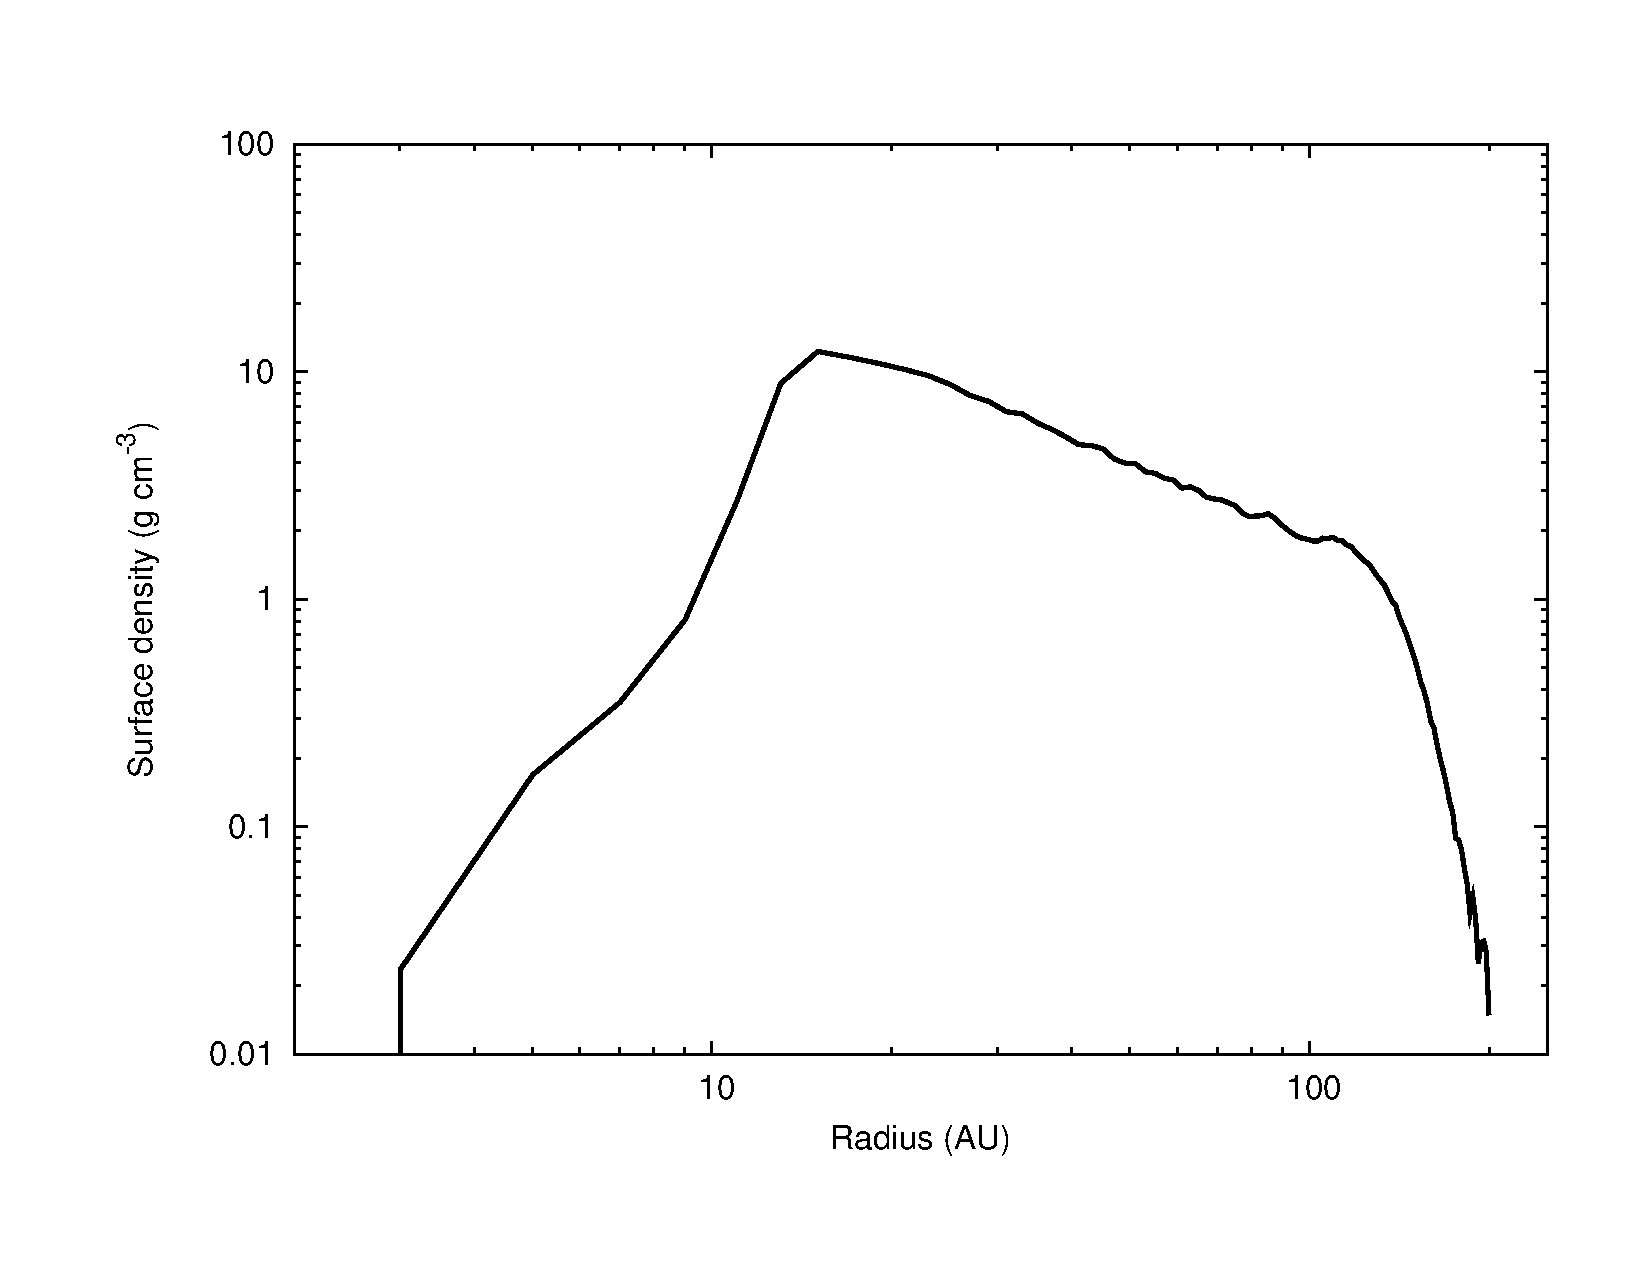
\includegraphics[scale=0.3]{figures/sigma_final}
  \caption{Surface density as a function of radius after 4986~years of simulated time.}
  \label{fig:sigma_final}
\end{figure}

The scale height of the disc was determined by fitting Gaussians to
the vertical density profile in 100 radial bins. The fitted scale
height, as a function of radius, is plotted in
Fig.~\ref{fig:scale_height}.  Within the central 10~AU the density
profile appears flat so it was not possible to fit a meaningful scale
height.
\begin{figure}
  \includegraphics[scale=0.3]{figures/scale_height}
  \caption{Disc scale height as a function of radius  after 4986~years of simulated time.}
  \label{fig:scale_height}
\end{figure}

The average temperature within one scale height of the disc mid plane
is plotted as a solid line in Fig.~\ref{fig:mid_tem}. The dashed line
is a power law variation of temperature with radius with an index of
$-0.35$. Although this line is not a formal best fit it has been
plotted to indicate that this temperature profile is well represented
by a power law outside 15AU.
\begin{figure}
  \includegraphics[scale=0.3]{figures/mid_tem}
  \caption{Average temperature within one scale height of the mid plane, as a function of
    radius, after 4986~years of simulated time.}
  \label{fig:mid_tem}
\end{figure}      

\section{Conclusions}

\label{section:conclusions}

We have presented results from a combined SPH and grid-based radiative
transfer code, which has been used to model a non-self gravitating
circumstellar disc. Validation tests of the method have revealed a
number of factors which must be taken into consideration when setting
up a model of this type. 

Although we have found a method for constructing an AMR grid from SPH
particles which is robust, in terms of the total mass on the grid, we
found that it was necessary to add additional grid refinement in the
central region of the disc to allow the inner edge to be well
represented. The inner edge of the disc has a disproportionately large
effect on the temperature distribution in the disc and on the emergent
SED. Consequently the accuracy of the solution is dependent upon the
accurate representation of a region which constitutes a small fraction
of the disc by volume. As the method combines both SPH and grid
elements it is important that both these components have sufficient
resolution to represent the disc inner edge. This presents a
particular challenge for a SPH code which uses equal mass particles
but is achievable with a large number of particles. 

The combined SPH-radiative transfer code was able to evolve a
circumstellar disc to a state of radiative and hydrostatic
equilibrium. Fluctuations in scale height were seen, which have also
been observed in codes which combine radiative transfer and vertical
hydrostatic equilibrium calculations. However there were also
transient effects seen in the surface density distribution which would
not be present if the hydrostatic equilibrium was calculated in the
vertical direction only. 

By adding self-gravity to the SPH model this method could be used to
explore the effects of radiative transfer on disc
fragmentation. However the model would need to be constructed
carefully to ensure sufficient resolution at the disc inner edge so
that the temperature distribution in the disc is accurate. Such a
model is expected to be feasible although computationally demanding. 

\section*{Acknowledgments}
Calculations presented here were performed using the University of
Exeter Supercomputer. DMA is funded by an EPSRC grant. 

\bibliographystyle{mn2e}
\bibliography{torus} 

\end{document}


